\documentclass[../main.tex]{subfiles} 

\begin{document}
\chapter{Identification of Suitable Hardware}
To select suitable \define{hardware} for a real-time embedded system we should first define what suitable means in this case. Suitable hardware is hardware that can satisfy the given (time) constraints and is not too overdimensioned.

\section{Select a maximal resource structure}

\begin{itemize}
	\item Each process executes on a different \define{processor} and has all the physical resource it needs.
	\item Processors are fast enough to satisfy the time constraints in this configuration. If the type of processor is predefined it should be verified that the processor can solve the given problems with a maximal resource structure. Else it means selecting one.
	\item Adding more resources of the same time is not useful
\end{itemize}

The following are properties of a maximal \define{resource} structure.
\begin{itemize}
	\item A process is never ``READY'' (never waiting for a process to run on): It's either ``RUNNING'' or ``WAITING'' (for an event or resource).
	\item The analysis of the worst case response time is easier to compute because processes don't interfere because of resource access conflicts. The only interferences are those dictated by the specification.
	\item It satisfies response time constraints if all the different stimuli occur simultaneously at boot time. And if there is no accumulation of debts from the past (calculations of a process finished before the next stimulus arrives).
\end{itemize}

\section{Reduce the structure by transformation}
Don't try to find the minimal structure (this problem is NP-complete) but a realistic solution. To do so, follow these to rules to restrict choices:
\begin{enumerate}
	\item No \define{process migration} (not a good idea in real-time)
	\item A processor is never idle if it can run one of the processes assigned to it.
\end{enumerate}

\begin{exmp}
\emph{Given is that:} 2 processes, P1 and P2, receive each an external stimulus (resp. x et y). After some pre-processing, they send the result to a process P3 that, after some processingn warns process P4, that reacts on the external system. 

\emph{Solution:} If we neglect message transmission times, one can represent what the 4 processes would do, on a maximal resource structure, if all stimuli occurred at boot time.
That gives us our (clearly correct) maximal resource structure as seen in \ref{f:sh_ex1}.
Not neglecting transmission times is an immediate adaptation of the representation. One can regroup P1 and P4 on a same processor, without lengthening the reaction times. It would also have been possible to regroup P2 and P4. Then the response time would have been increased, but would still satisfy the constraint.
As, in normal working conditions (thus without taking initialization into account), P2 is working the most, it will be P2 that will determine the lowest possible repetition period of the stimuli (duration of pre-processing + post-processing of P2). However, at that rate, no grouping of processes is possible anymore.

\begin{figure}[H]
	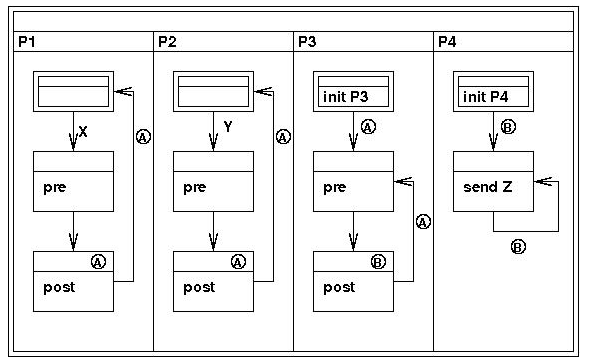
\includegraphics{Suitable_Hardware_ex1.png}
	\caption{Figure representing the maximal resource structure of the given problem.}
	\label{f:sh_ex1}
\end{figure}

\begin{figure}[H]
	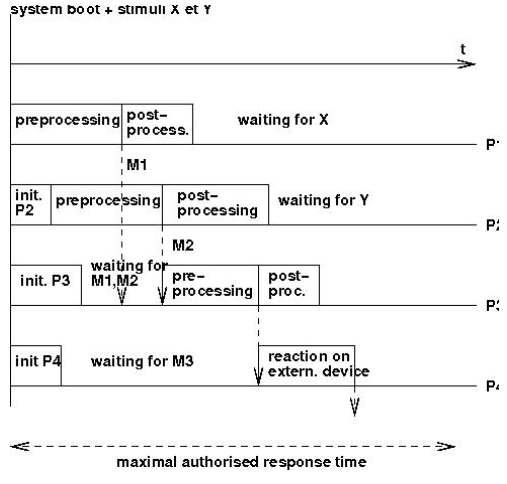
\includegraphics{Suitable_Hardware_ex2.png}
	\caption{Figure representing the maximal resource structure of the given problem.}
	\label{f:sh_ex2}
\end{figure}
\end{exmp}



\end{document}
